Dialog System Technology Challenges 8 (DSTC8) \cite{dstc8}とは対話に関するコンペティションである.2013 年に最初の Dialog State Tracking Challenge(対話状態追跡タスク)が開催された.第 6 回から対話状態追跡だけでなく,対話破綻検出や応答生成といった対象となるタスクの幅が広がり,略称はDSTCのままで現在の Dialog System Technology Challenges へと名称が変更された.
\par
ここでは本研究で取り組んだ対話状態追跡タスクの DSTC8-Track4 について説明する.昨今,ホテル案内や交通案内などのドメインを行えるサービスが多く存在している.サービスごとに様々な バックエンドAPI が定義されるため,同じドメインでもシステムが理解できず,対応させるには再学習が必要となる.
DSTC8-Track4では,現在の対話システムの課題の1つである新サービスへの拡張を再学習なしで可能にすることを目的としており,そのための対話状態追跡モデルを作成する.
\par
本タスクでは,ユーザが対話で達成したい目的をインテントと呼ぶ.インテントはサービスごとにいくつか存在する.例えばレストランサービスであれば,レストラン検索(FindRestaurant)とレストラン予約(ReserveRestaurant)が存在する.システムはサービスに対応するインテントの変化を追跡することで,ユーザの目的に合った質問や返答を返すことが可能になる.
\par
また,本タスクではサービスを定義する枠組みであるスキーマが用意されている.スキーマは,サービスごとにスロットのリストとインテントのリストを持つ.スキーマの構成は図\ref{fig:schema}に示す.
\begin{figure}[thb]
    \centering
    \includegraphics[width=15cm]{chapter2/schema2.eps}
    \caption{スキーマの構成}
    \label{fig:schema}
\end{figure}
スキーマには,サービス,スロット,インテント全てに説明文が付与されている.この説明文によって,システムが未知のサービス,スロット,インテントを理解することを可能にする.スロットに関してはスロット値候補を持つ候補ありスロットと,候補を持たない候補なしスロットに分けられる.候補ありスロットはスロット値を事前に与えられている候補から選択するが,候補なしスロットはスロット値を発話文中から抜き出す必要がある.図\ref{fig:schema}では,乗り換えの回数を表す“number\_stops”スロット,航空会社を表す“airlines”が候補ありスロット,出発地を表す“origin”スロット,到着地を表す“destination”スロットなどそれ以外が候補なしスロットにあたる.また,各インテントの達成に必要なスロットという情報を持つため,システムはスキーマによってサービスの バックエンドAPI が何を必要としているかを理解できる.
\par
\begin{figure}[t]
    \centering
    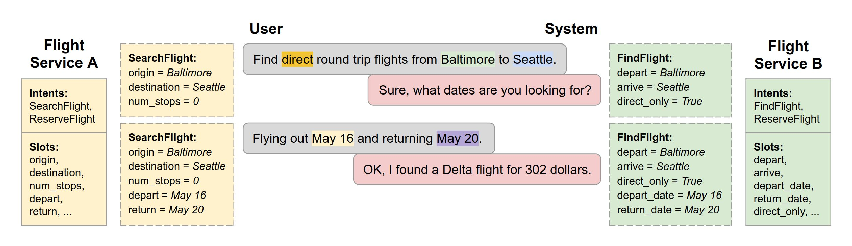
\includegraphics[width=15cm]{chapter2/dstc8-track4.eps}
    \caption{DSTC8-Track4 のイメージ図\cite{dstc8}}
    \label{fig:dstc8-track4}
\end{figure}
本タスクは,学習時,検証時,テスト時それぞれで扱うサービスが異なる.図\ref{fig:dstc8-track4}に示した通り,同じ “Flight Service” でもインテントの候補とスロットが異なる名前で定義されている.そして,どちらのサービスを扱うとしても,ユーザの目的と要求を同様に推定できる対話状態追跡モデルを作成する必要がある.
\par 
参加者はベースラインモデルと整形された対話データセットが配布され,そのデータセットなどを用いて作成したモデルの学習と評価を行い,モデルと評価結果を提出する.
\par 
配布されたデータセットは SGD データセットと呼ばれ,人とシステムの間のラベル付きタスク指向型対話を持つ.各対話はユーザとシステムが交互に 1 発話ずつ行い,1 発話につき 1 ターンとしている.1 ターンごとに,発話中に存在するスロット値候補の位置を範囲で示すスロット値範囲リストが与えられる.スロット値範囲リストは以下の要素を持つ.
\begin{itemize}
    \item スロット - スロットの名前
    \item 開始位置 - 発話中にあるスロット値候補の開始位置
    \item 終了位置 - 発話中にあるスロット値候補の終了位置
\end{itemize}
対話状態はユーザのターンのみ与えられる.対話状態は以下の要素を持つ.
\begin{itemize}
    \item インテント(Noneを含む)
    \item 要求スロット - ユーザが値を要求しているスロットのリスト
    \item スロット値 - 各スロットに当てはまる値
\end{itemize}
対話状態の推定は,この3つの要素を全て推定する必要がある.
また,対話行為はシステムのターンのみ与えられる.本タスクの対話行為は,システムがあるスロットに対してどのような行動をしたのかを示すため,以下の要素を持つ.
\begin{itemize}
    \item 対話行為タグ - 対話行為の種類を示す
    \item スロット - 対話行為が関与しているスロット
    \item スロット値 - 対話行為で用いたスロット値
\end{itemize}
例えば “OFFER (origin, Baltimore)” ならば,出発地として “Baltimore” を提案するという行動を示す.
\par
本タスクでは,発話文,スキーマ,対話行為を入力として,対話状態であるインテント,要求スロット,スロット値を推定する.スロット値に関して,候補ありスロットではスロット値をスキーマから与えられるスロット値候補から推定し,候補なしスロットではスロット値となる文字列の範囲を発話中から推定する.候補なしスロットの推定では,既にスロットに割り当てられている値と同じ意味の値(例:“at afternoon 1:30”, “1:30 pm”)を推定することがあるため,候補なしスロットには複数の値が割り当てられることもある.